\ifdefined\HANDOUTMODE
	% handout: final overlay + notes
	% buggy sometimes because minted blocks can't be easily wrapped
	\documentclass[handout, aspectratio=169, 10pt]{beamer}
  	\setbeameroption{show notes}    
\else
	% normal presentation
	\documentclass[aspectratio=169, 10pt]{beamer}
	% notes are automatically suppressed
\fi

% Change language to german
%\usepackage[utf8]{inputenc}
%\usepackage[T1]{fontenc}
%\usepackage[ngerman]{babel}

% References
\usepackage[backend=biber,style=ieee]{biblatex}
\addbibresource{references.bib}

% Theme
\usetheme{gotham}

% Reset font sizes to allow changing fullsize font size
\setbeamerfont{bibliography entry title}{size=}
\setbeamerfont{bibliography entry author}{size=}
\setbeamerfont{bibliography entry location}{size=}
\setbeamerfont{bibliography entry note}{size=}

\gothamset{
	% Defaults
	background=transparent,
	block=native,
	%numbering= framenumber,
	parttocframe default=off,
	sectiontocframe default=off,
	subsectiontocframe default=off,
	% Custom
	tocframe template= gotham simple,
	%progressbar position=foot,
	numbering= totalframenumber,
}

% Custom ToC for less spacing between sections
\makeatletter
\def\beamer@sectionintoc#1#2#3#4#5{%
	\vspace{0.35em}%
	\leavevmode
	\leftskip=1.5em
	\usebeamerfont{section number projected}#1\hspace{0.75em}%
	\usebeamerfont{section in toc}#2\par
}
\makeatother

\usepackage{standalone}
\usepackage{tikz}
\usetikzlibrary{automata, positioning}
%\usepackage{pgfplots}
\usepackage{tabularray} % Typeset tabulars and arrays (contains equivalent of longtable, booktabs and dcolumn at least)
	\UseTblrLibrary{booktabs} % to load extra commands from booktabs
\usepackage{changepage}
\usepackage{appendixnumberbeamer}
	\newcommand{\famName}[1]{\textsc{#1}}
\usepackage{minted}
	\definecolor{codeback}{rgb}{0.90,0.91,0.92}
	\definecolor{codebackdark}{rgb}{0.10,0.11,0.12}
	\usemintedstyle{emacs}
	\setmintedinline[tex]{bgcolor=codeback}
	\setminted[tex]{
		autogobble,
		bgcolor=codeback,
		tabsize=4,
		extrakeywords={usetheme,institute,maketitle,subtitle,gothamset,colorlet,setbeamercolor,plain,defbeamertemplate}
	}

\usepackage[scale=2]{ccicons}
%\usepackage{pgfplots}
%\usepgfplotslibrary{dateplot}
\usepackage{colortbl} % alternating table colors

% Footnote without a marker (https://tex.stackexchange.com/a/30726)
\newcommand\blfootnote[1]{%
  \begingroup
  \renewcommand\thefootnote{}\footnote{#1}%
  \addtocounter{footnote}{-1}%
  \endgroup
}

\newcommand{\themename}{\textbf{\textsc{Gotham}}}
\newcommand{\patternname}{RAII - Resource Acquisition Is Initialization}

\title[]{\patternname}
\subtitle{Example Title}
\date[]{2026.01.09}
\author[]{Your Name \textless{your@email.de}\textgreater}
\institute{HdM Stuttgart}
%\titlegraphic{\hfill\includegraphics[height=1.5cm]{res/HdM_Logo.pdf}}

% Make printbibliography smaller
\renewcommand*{\bibfont}{\footnotesize}

\begin{document}

\maketitle

\begin{frame}{Introduction}
	\begin{figure}
		\centering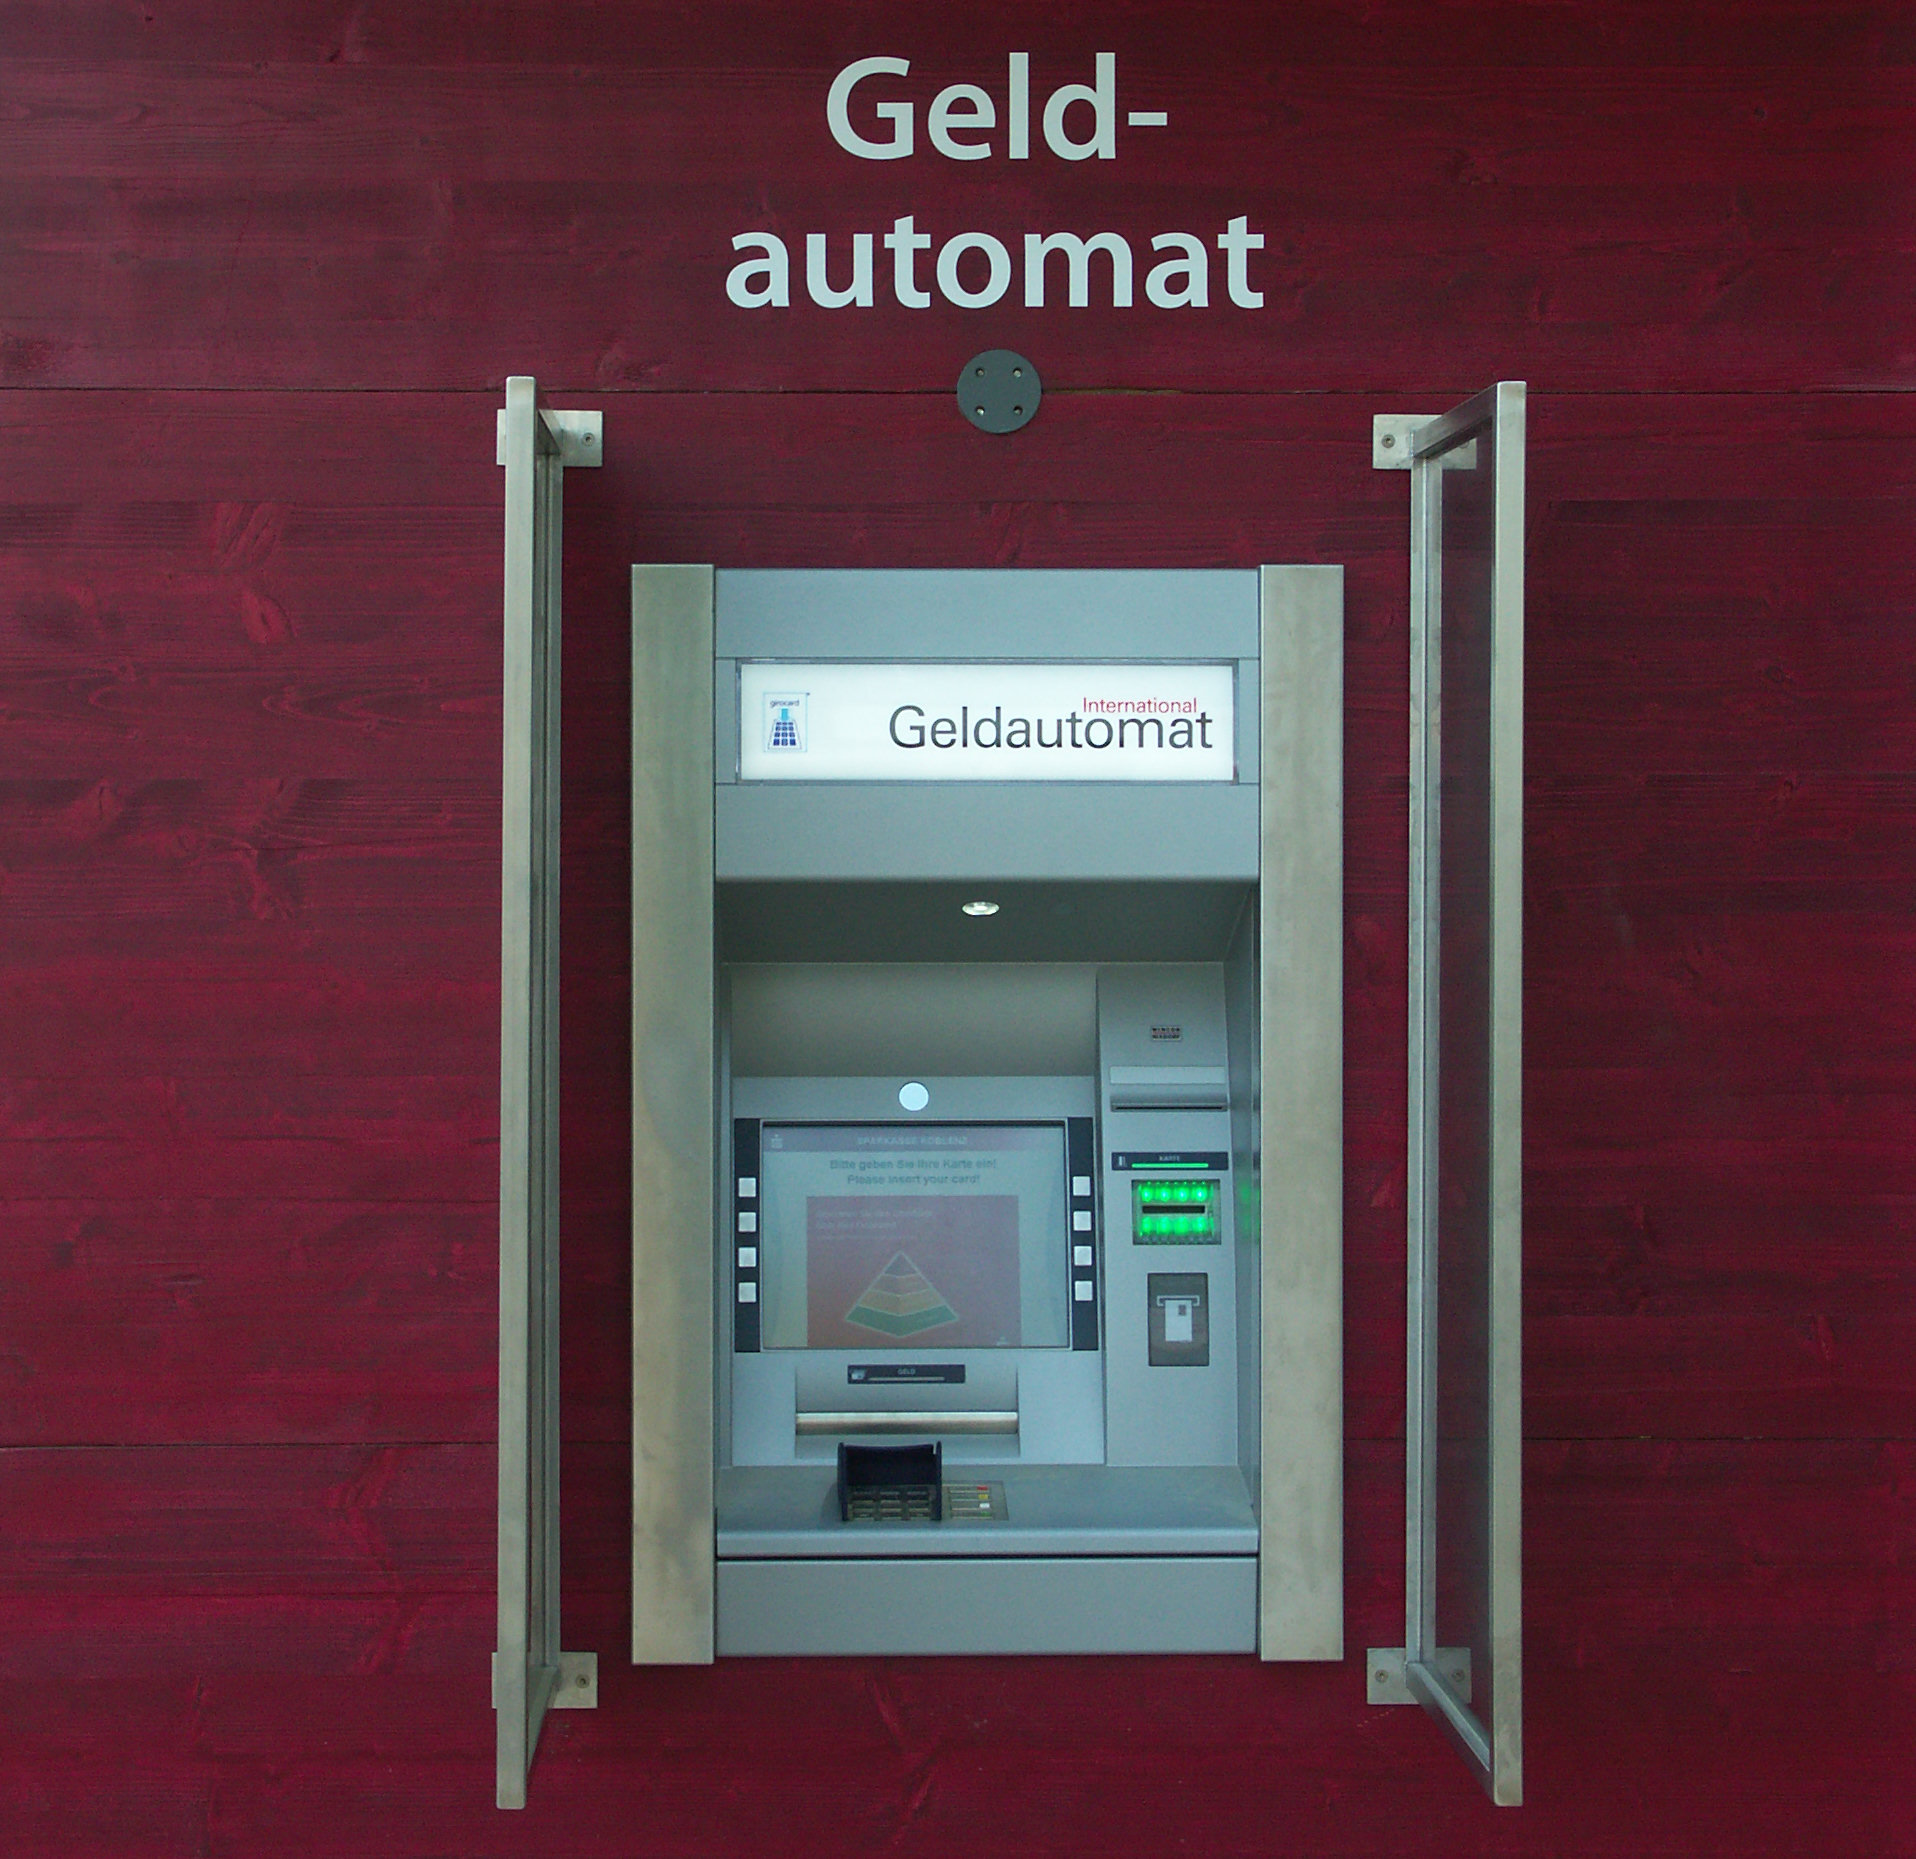
\includegraphics[height=0.7\textheight]{res/wikimedia_geldautomat.jpg}
		\caption{Geldautomat/ATM (or Kontoauszugsautomat/Bank Statement Printer) \newline \tiny \fullcite{wikimedia_image_geldautomat}}
	\end{figure}

	\note{
		Question: Describe the process of withdrawing money on an ATM?
	}
\end{frame}

\begin{frame}{RAII Concept: ATM Example}
	\centering
	\definecolor{gothamYellow}{HTML}{FFCC00} % ignore last FF, LaTeX hex only takes RRGGBB
	\begin{tikzpicture}[
			>=stealth,
			node distance=6cm,
			% Reduce the font size of nodes and labels
			every node/.style = {font=\footnotesize},
			every label/.style = {font=\footnotesize},
			% Specify default state
			every state/.style={thick, minimum size=8mm, align=center},
			% Specify highlighted state
			highlight/.style={draw=gothamYellow, very thick, fill=gothamYellow!30},
		]

		% States
		% > Top row
		\node[state, highlight] (cardInserted) {
			Insert card\\
			(Acquire resource)
		};
		\node[state, right=4cm of cardInserted] (withdraw) {
			Withdraw money/\\bank statements
		};
		% > Bottom row
		\node[state, highlight, below=1cm of withdraw] (returnCard) {
			Return card\\
			(Release resource)
		};
		\node[state, left=4cm of returnCard] (dispense) {
			Dispense money/\\bank statements
		};

		% Transitions
		\draw[->, thick] (cardInserted) -- (withdraw) node[midway, above, align=center] {
			Enter PIN / Authenticate\\
			(Use resource)
		};
		\draw[->, thick] (withdraw) -- (returnCard) node[midway, right, align=center] {};
		\draw[->, thick] (returnCard) -- (dispense) node[midway, above, align=center] {};

	\end{tikzpicture}

	\note{
		Important discovery:
		\begin{itemize}
			\item Card is returned before the \textit{goal} of taking the money is reached
			\item Pattern RAII connects a resource (bank card) to the lifetime of the process to not accidentally forget it
		\end{itemize}
	}
\end{frame}


\begin{frame}[toc]{Table of Contents (\patternname)}
	\tableofcontents[hideallsubsections]
	% Don't include subsections for simpler visuals
	%\tableofcontents%[hideallsubsections]
\end{frame}

\section{Anti-Pattern}

% FRAME
\begin{frame}[fragile]{Anti-Pattern: Manual Resource Management}
	\begin{tikzpicture}[remember picture,overlay]
		\begin{onlyenv}<2->
			\node at (current page.south east) [xshift=-3.5cm, yshift=5.8cm]
			{
\includegraphics[width=1.5cm]{res/nuke.pdf}};
		\end{onlyenv}
		\begin{onlyenv}<3->
			\node at (current page.south east) [xshift=-2cm, yshift=3.2cm]
			{
\includegraphics[width=1.5cm]{res/nuke.pdf}};
		\end{onlyenv}
	\end{tikzpicture}
	\begin{figure}
		\centering
		\begin{minipage}{0.8\linewidth}
			\vspace{-5mm}
			\begin{onlyenv}<1>
				\vspace{0.1cm}
				\begin{minted}{py}
def read_file():
    f = open("data.txt", "r")
    content = f.read()

    return content
            \end{minted}
			\end{onlyenv}
			\begin{onlyenv}<2->
				\begin{minted}{py}
def read_file():
    f = open("data.txt", "r")
    content = f.read()
    # f.close();  <-- Oops, never closed!
    return content
            \end{minted}
			\end{onlyenv}
			\begin{onlyenv}<1-2>
				\rule{\linewidth}{0.5mm}
				\begin{minted}{java}
public String getString() {
    Scanner scanner = new Scanner(System.in);
    String name = scanner.nextLine();

    return name;
}
            \end{minted}
			\end{onlyenv}
			\begin{onlyenv}<3->
				\rule{\linewidth}{0.5mm}
				\begin{minted}{java}
public String getString() {
    Scanner scanner = new Scanner(System.in);
    String name = scanner.nextLine();
    // scanner.close();  <-- Oops, never closed!
    return name;
}
            \end{minted}
			\end{onlyenv}
		\end{minipage}
		\caption{Example: Manual Resource Management in Python/Java}
	\end{figure}
\end{frame}

\begin{frame}[fragile]{Reminder: Memory Management Model Differences}
	\begin{tikzpicture}[remember picture,overlay]
		\only{
			\node at (current page.south east) [xshift=-6.75cm, yshift=3.75cm]
			{
\includegraphics[width=0.6cm]{res/nuke.pdf}};
			\node at (current page.south east) [xshift=-7.5cm, yshift=3.75cm]
			{
\includegraphics[width=0.6cm]{res/nuke.pdf}};
		}<2->
		\only{
			\node at (current page.south east) [xshift=-2cm, yshift=1.25cm]
			{
\includegraphics[width=1.4cm]{res/nuke.pdf}};
			\node at (current page.south east) [xshift=-3cm, yshift=1.25cm]
			{
\includegraphics[width=1.4cm]{res/nuke.pdf}};
			\node at (current page.south east) [xshift=-4cm, yshift=1.25cm]
			{
\includegraphics[width=1.4cm]{res/nuke.pdf}};
		}<4->
	\end{tikzpicture}
	\vspace{-1cm}
	\begin{itemize}
		\item \textbf{Java}: (Memory-Safe)
		      \begin{itemize}
			      \item Objects are allocated on the heap\footnote{Escape Analysis can enable stack allocation \cite{oracle_jvm_guide_jdk24}} and accessed via references (\mintinline{java}|new|)
			      \item The JVM Garbage Collector determines whether objects are still reachable via references
			            \begin{itemize}
				            \item Possibly pausing execution at non-deterministic points
				            \item Unreachable objects are reclaimed automatically (their memory)
			            \end{itemize}
			      \item Array bounds and pointer dereferences are checked at runtime
			      \item Memory errors are limited to logical issues:
			            \begin{itemize}
				            \item \mintinline{java}|ArrayIndexOutOfBoundsException|
				            \item \mintinline{java}|NullPointerException|
			            \end{itemize}
		      \end{itemize}
		\item<3-> \textbf{C/C++}: (Memory-Unsafe)
		      \begin{itemize}
			      \item Memory (on the heap) is allocated \textbf{and freed} explicitly (\mintinline{c}|malloc|/\mintinline{c}|free|, \mintinline{cpp}|new|/\mintinline{cpp}|delete|)
			      \item \textbf{No} runtime checks (e.g. array bounds, pointer dereferences)
			      \item \textbf{Direct and unchecked} memory access
		      \end{itemize}
	\end{itemize}
\end{frame}

\begin{frame}[fragile]{Anti-Pattern: Manual Memory Management (i)}
	\begin{tikzpicture}[remember picture,overlay]
		\node at (current page.south east) [xshift=-3cm, yshift=6.3cm]
		{
\includegraphics[width=1.5cm]{res/nuke.pdf}};
		\only{
			\node at (current page.south east) [xshift=-1.25cm, yshift=3.5cm]
			{
\includegraphics[width=1.5cm]{res/nuke.pdf}};
		}<2->
		\only{
			\node at (current page.south east) [xshift=-3cm, yshift=0.9cm]
			{
\includegraphics[width=1.5cm]{res/nuke.pdf}};
		}<3->
	\end{tikzpicture}
	\begin{figure}
		\centering
		\begin{minipage}{0.8\linewidth}
			\begin{minted}{c}
int *numbers = malloc(5 * sizeof(int));
for (int i = 0; i < 5; i++) {
	numbers[i] = i * 10;
}
// free(numbers);  <-- Memory never given back (Memory Leak)
			\end{minted}
			\begin{onlyenv}<-1>
				\vspace{1.65cm}
			\end{onlyenv}
			\begin{onlyenv}<2->
				\rule{\linewidth}{0.5mm}
				\begin{minted}{c}
free(numbers);
free(numbers); // <-- Memory given back twice! (Double-Free)
				\end{minted}
			\end{onlyenv}
			\begin{onlyenv}<-2>
				\vspace{1.55cm}
			\end{onlyenv}
			\begin{onlyenv}<3->
				\rule{\linewidth}{0.5mm}
				\begin{minted}{c}
free(numbers); // dangling pointer referencing invalid memory
printf("%d\n", numbers[0]); // <-- Use after free!
				\end{minted}
			\end{onlyenv}
		\end{minipage}
		\caption{Example: Manual Memory Management in C}
	\end{figure}
	\vspace{-1cm}
	\blfootnote{\cite{CWE401} \cite{CWE415} \cite{CWE416}}
\end{frame}

\begin{frame}[fragile]{Anti-Pattern: Manual Memory Management (ii)}
	\begin{tikzpicture}[remember picture,overlay]
		\node at (current page.south east) [xshift=-4cm, yshift=4cm]
		{
\includegraphics[width=1.5cm]{res/nuke.pdf}};
	\end{tikzpicture}
	\begin{figure}
		\centering
		\begin{minipage}{0.8\linewidth}
			\begin{minted}{cpp}
int *numbers = malloc(5 * sizeof(int));
for (int i = 0; i < 5; i++) {
	numbers[i] = i * 10;
}
throw std::runtime_error("simulated error");
free(buf); // <-- Memory never given back
			\end{minted}
		\end{minipage}
		\caption{Example: Manual Memory Management in C++ (with Exceptions)}
	\end{figure}
	\blfootnote{\cite{isocpp_coreguidelines}}
\end{frame}


\section{Pattern Description}

\begin{frame}[fragile]{History of \patternname}
	\begin{columns}[T,onlytextwidth]
		\begin{column}{0.6\textwidth}
			\begin{itemize}
				\item Introduction by Bjarne Stroustrup in the early 1990s as part of C++ design
				      \begin{itemize}
					      \item Programming Idiom: \textit{Common, conventional way of writing code to solve a recurring problem}
				      \end{itemize}
				\item Its purpose is to \textbf{bind resource management to object lifetime}
				      \begin{itemize}
					      \item Resources (memory, files, locks) are \textbf{acquired in Constructors}
					      \item Resources are guaranteed to be \textbf{automatically released in Destructors} (Deterministic)
				      \end{itemize}
				\item Safer code at essentially zero runtime overhead
				      \begin{itemize}
					      \item Memory-Safety
					      \item Exception-Safety
				      \end{itemize}
			\end{itemize}
		\end{column}
		\begin{column}{0.4\textwidth}
			\begin{figure}
				\centering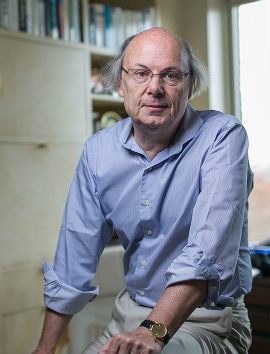
\includegraphics[height=0.5\textheight]{res/Bjarne2018.jpg}
				\caption{Bjarne Stroustrup \newline \tiny \fullcite{stroustrup_image}}
			\end{figure}
		\end{column}
	\end{columns}
	\blfootnote{\cite{cppreference_raii} \cite{isocpp_coreguidelines} \cite{Stroustrup2018-ic} \cite{Will2020-og} \cite{Meyers2014-ot}}
\end{frame}



\begin{frame}[fragile]{\patternname\ (i)}
	\begin{columns}[T,onlytextwidth]
		\begin{column}{0.6\textwidth}
			\begin{itemize}
				\item Idea:
				      \begin{itemize}
					      \item No manual \mintinline{cpp}|new|
					      \item No manual \mintinline{cpp}|delete|/\mintinline{cpp}|delete[]|
				      \end{itemize}
				\item Constructor: Initializes and Acquires Resources
				\item \textbf{Destructor}: Releases all Acquired Resources
				      \begin{itemize}
					      \item Automatically:
					            \begin{itemize}
						            \item Out of scope
						            \item Exception is thrown
					            \end{itemize}
					      \item Guaranteed by the programming language
				      \end{itemize}
			\end{itemize}
		\end{column}
		\begin{column}{0.4\textwidth}
			\begin{figure}
				\centering
				\begin{minted}{cpp}
int main() {
    int* arr = new int[10];
    // ...
    delete[] arr; // manual!
} // not exception safe!
                \end{minted}
				\rule{\linewidth}{0.5mm}
				\begin{minted}{cpp}
#include <vector>
int main() {
    std::vector<int> arr(10);
    // ...
} // automatic release
                \end{minted}
				\caption{Example: RAII vs Manual Memory Management, Array with 10 Integers on the Heap}
			\end{figure}
		\end{column}
	\end{columns}
\end{frame}

\begin{frame}[fragile]{\patternname\ (ii)}
	\begin{figure}
		\centering
		\begin{minted}{cpp}
class MyClass {
	int* m_arr;
public:
	MyClass() { // Constructor: Create Object (explicit)
		m_arr = new int[10];
	}
	~MyClass() { // Destructor: Delete Object (automatically)
		delete[] m_arr;
	}
};
int main() {
	MyClass obj; // Constructor
} // Destructor automatically runs at the end of scope
  // Even when an exception is thrown!
	    \end{minted}
		\caption{Example: RAII implementation}
	\end{figure}
\end{frame}

% TODO References!


\section{Problems and Shortcomings}

\begin{frame}[fragile]{Problem: RAII Is not the default}
	\begin{columns}[T,onlytextwidth]
		\begin{column}{0.35\textwidth}
			\begin{itemize}
				\item Programmers need to be aware of the pattern
				\item The Standard Library implements RAII but it's not required for other libraries or C libraries which often require RAII wrappers:
				      \begin{itemize}
					      \item Container
					      \item Smart Pointer
					      \item Lock Guard
				      \end{itemize}
			\end{itemize}
		\end{column}
		\begin{column}{0.6\textwidth}
			\begin{figure}
				\centering
				\begin{minted}{cpp}
struct Resource {};
int main() {
    Resource* r = new Resource();
    delete r; // RAII not automatic
}
                \end{minted}
				\rule{\linewidth}{0.5mm}
				\begin{minted}{cpp}
#include <memory>
struct Resource {};
int main() {
    auto s = std::make_unique<Resource>();
}  // RAII automatic
                \end{minted}
				\caption{Example: C++ RAII is not the default}
			\end{figure}
		\end{column}
	\end{columns}
	\blfootnote{\cite{Stroustrup2018-ic} \cite{Meyers2014-ot}}
\end{frame}

\begin{frame}[fragile]{Problem: Ownership Issues}
	\begin{columns}[T,onlytextwidth]
		\begin{column}{0.37\textwidth}
			\begin{itemize}
				\item Rule of Three (Copy)
				      \begin{enumerate}
					      \item \textbf{Destructor: release resource}
					      \item \textit{Copy} constructor: Copy the resource safely
					      \item \textit{Copy} assignment operator
				      \end{enumerate}
				\item Rule of Five (Move)
				      \begin{enumerate}\setcounter{enumi}{3}
					      \item \textit{Move} constructor: Transfer ownership safely
					      \item \textit{Move} assignment operator
				      \end{enumerate}
				\item Reference Counting
				      \begin{itemize}
					      \item \mintinline{cpp}|std::shared_ptr|
					      \item \mintinline{cpp}|std::weak_ptr|
				      \end{itemize}
			\end{itemize}
		\end{column}
		\begin{column}{0.58\textwidth}
			\begin{figure}
				\centering
				\begin{minted}{cpp}
#include <cstring>
struct Buffer {
    char* data;
    Buffer(const char* s) {
        data = new char[strlen(s)+1];
        strcpy(data, s);
    }
    ~Buffer() { delete[] data; }
};
int main() {
    Buffer a("Hello");
    Buffer b = a; // default copy: shallow copy
} // a and b both run Destructor: double free
                \end{minted}
				\caption{Example: C++ RAII Rule of Three reason}
			\end{figure}
		\end{column}
	\end{columns}
	\vspace{-1cm}
	\blfootnote{\cite{Meyers2014-ot} \cite{isocpp_coreguidelines}}
\end{frame}

\begin{frame}[fragile]{Problem: Cyclic References}
	\begin{columns}[T,onlytextwidth]
		\begin{column}{0.35\textwidth}
			\begin{itemize}
				\item RAII Destructors may not run if objects reference each other
				\item \textit{A Garbage Collector can actually detect that both nodes are not referenced since it doesn't rely on reference counting}
			\end{itemize}
		\end{column}
		\begin{column}{0.6\textwidth}
			\begin{figure}
				\centering
				\begin{minted}{cpp}
#include <memory>
struct Node {
    std::shared_ptr<Node> next;
};
int main() {
    auto a = std::make_shared<Node>();
    auto b = std::make_shared<Node>();
    a->next = b;
    b->next = a;
} // cycle: memory leak
                \end{minted}
				\caption{Example: C++ Cyclic References break RAII}
			\end{figure}
		\end{column}
	\end{columns}
\end{frame}

\begin{frame}[fragile]{Problem: Inheritance Issues}
	\begin{columns}[T,onlytextwidth]
		\begin{column}{0.35\textwidth}
			\begin{itemize}
				\item \mintinline{cpp}|Derived|'s Destructor is never called because \mintinline{cpp}|Base|'s Destructor is not \mintinline{cpp}|virtual|
				\item Performance/Memory overhead: \mintinline{cpp}|virtual| introduces a small runtime (dynamic dispatch) and memory (alignment) cost because of a pointer on each object and a class vtable
			\end{itemize}
		\end{column}
		\begin{column}{0.6\textwidth}
			\begin{figure}
				\centering
				\begin{minted}{cpp}
class Base {
public:
                  Base() {}
    /* virtual */ ~Base() {}
};
class Derived : public Base {
public:
    Derived() {}
    ~Derived() {}
};
int main() {
    Base* obj = new Derived();
} // only Base Destructor is called!
                \end{minted}
				\caption{Example: C++ RAII virtual importance}
			\end{figure}
		\end{column}
	\end{columns}
\end{frame}


\section{Other Implementations}

\begin{frame}[fragile]{Java (try-with-resources)}
	\begin{columns}[T,onlytextwidth]
		\begin{column}{0.35\textwidth}
			\begin{itemize}
				\item Requires
				      \begin{itemize}
					      \item Interface implementation (\mintinline{java}|AutoCloseable|)
					      \item Being inside a \mintinline{java}|try| block
				      \end{itemize}
				\item Java guarantees calling \mintinline{java}|close()| in a generated \mintinline{java}|final| block and nothing else
				\item Exception safe
				\item Release of actual memory requires waiting for Garbage Collector pause (Non-Deterministic)
			\end{itemize}
		\end{column}
		\begin{column}{0.6\textwidth}
			\begin{figure}
				\centering
				\begin{minted}{java}
class Demo implements AutoCloseable {
    Demo() { /* Constructor */ }
    @Override
    public void close() {
        /* 'Destructor' */
    }
    public static void main(String[] args) {
        try (Demo d = new Demo()) {
            // ...
        } // close() is automatically called
    }
}
                \end{minted}
				\caption{Example: Java implementation of RAII}
			\end{figure}
		\end{column}
	\end{columns}
	\blfootnote{\cite{oracle_try_with_resources}}
\end{frame}

\begin{frame}[fragile]{Rust (Drop)}
	\begin{columns}[T,onlytextwidth]
		\begin{column}{0.45\textwidth}
			\begin{itemize}
				\item RAII is a core principle of the language rather than a pattern you opt into:
				      \begin{itemize}
					      \item Rust has no delete
				      \end{itemize}
				\item Ownership system:
				      \begin{itemize}
					      \item Every value has one owner
					      \item When the owner goes out of scope, the value is dropped
					      \item Cleanup logic is placed in the \mintinline{rust}|Drop| trait
				      \end{itemize}
			\end{itemize}
		\end{column}
		\begin{column}{0.5\textwidth}
			\begin{figure}
				\centering
				\begin{minted}{rust}
struct Demo;
impl Drop for Demo {
    fn drop(&mut self) { /* ... */ }
}
fn main() {
    let d = Demo;
} // drop() is called automatically
                \end{minted}
				\rule{\linewidth}{0.5mm}
				\begin{minted}{rust}
let a = String::from("data");
let b = a; // ownership moved to b
// only b will be dropped, a invalid
                \end{minted}
				\caption{Example: Rust implementation of RAII}
			\end{figure}
		\end{column}
	\end{columns}
	\blfootnote{\cite{rust_drop_trait}}
\end{frame}

\begin{frame}{Implementation Comparison Summary}
	\rowcolors{2}{gray!10}{white}

	\begin{table}
		\centering
		\renewcommand{\arraystretch}{1.3}
		\begin{tabular}{l p{3cm} p{3cm} p{3cm}}
			\textbf{Aspect} & \textbf{C++}                                                                   & \textbf{Java} & \textbf{Rust} \\ \hline

			Automatic everywhere
			                & \textcolor{green!60!black}{Yes}
			                & \textcolor{orange}{Limited (only in \mintinline{java}|try| blocks)}
			                & \textcolor{green!60!black}{Yes}                                                                                \\

			Deterministic destruction
			                & \textcolor{green!60!black}{Yes}
			                & \textcolor{orange}{Limited (still needs to wait for GC)}
			                & \textcolor{green!60!black}{Yes}                                                                                \\

			Exception safe
			                & \textcolor{green!60!black}{Yes}
			                & \textcolor{green!60!black}{Yes}
			                & \textcolor{green!60!black}{Yes}                                                                                \\

			Compiler enforcement
			                & \textcolor{orange}{Partial (many mistakes possible in implementation)}
			                & \textcolor{red}{Minimal (only guarantees the \mintinline{java}|close{}| call)}
			                & \textcolor{green!60!black}{Strong (also enforces ownership, borrowing, ...)}                                   \\
		\end{tabular}
	\end{table}

	\vspace{0.5em}
	\footnotesize
	\textit{* GC = Garbage Collector}
\end{frame}


\section{Questions}
\addtocounter{framenumber}{1} % manually increment since standoutenv doesn't do it


\section{Discussion}

% FRAME
\begin{standoutenv}
	\begin{frame}[fragile]
		\begin{enumerate}
			\item<1-> Has anyone worked with memory unsafe languages before, and if yes what was your experience regarding memory/resource management?
			\item<2-> RAII automates cleanup but is automation always better than manual intervention or when is it a bad idea?
			\item<3-> What real-life systems, habits or patterns do you rely on to manage resources (like time, energy, ...) or maybe even unexpected interruptions/distractions?
			\item<4-> Do you use or know any other patterns in programming languages or software to manage resources?
		\end{enumerate}

		\note{
			\begin{itemize}
				\item Segmentation Fault
				\item Reliability and safety, Predictability, Time and cognitive savings but Performance overhead, Loss of flexibility, Unexpected side effects
				\item Timers: Cooking Top, Pomodoro
				\item Python context manager
			\end{itemize}
		}
	\end{frame}
\end{standoutenv}
\addtocounter{framenumber}{1} % manually increment since standoutenv doesn't do it


\section{References and Credits}

\begin{frame}[allowframebreaks]{References}
	\printbibliography[heading=none]
\end{frame}

\begin{frame}[allowframebreaks]{Credits}
	\footnotesize
	This presentation was created using \textbf{latexmk} and \textbf{biber} using the theme \textbf{beamertheme-gotham} maintained by Romain NOËL,
	available at \url{https://gitlab.com/RomainNOEL/beamertheme-gotham},
	licensed under the \textit{LPPL Version 1.3c}.

	The nuke cartoon image is part of the public domain published on \url{https://freesvg.org/nuclear-explosion-drawing} by OpenClipart (downloaded on the 28.11.2025).

	The introduction idea with the ATM and bank card was inspired by Dr. Patrick Bader's lecture \textit{Advanced Programming in C++} at the HdM Stuttgart.
\end{frame}

\appendix

\begin{frame}[fragile]{Backup: Python Implementation of RAII}
	\begin{figure}
		\centering
		\begin{columns}[T,onlytextwidth]
			\begin{column}{0.5\textwidth}
				\begin{minted}{py}
def read_file():
    f = open("data.txt", "r")
    content = f.read()
    return content
		\end{minted}
				\rule{\linewidth}{0.5mm}
				\begin{minted}{py}
def read_file():
    with open("data.txt", "r") as f:
        content = f.read()
    return content
				\end{minted}
			\end{column}
			\begin{column}{0.5\textwidth}
				\begin{minted}{py}
class FileReader:
    def __init__(self, path):
        self.file = open(path, "r")
    def read(self):
        return self.file.read()
    def __del__(self):
        if not self.file.closed:
            self.file.close()
def read_file():
    reader = FileReader("data.txt")
    return reader.read()
				\end{minted}
			\end{column}
		\end{columns}
		\caption{Example: RAII concepts in Python}
	\end{figure}
\end{frame}

\begin{frame}[fragile]{Backup: C++ Lock Guard}
	\begin{figure}
		\centering
		\begin{columns}[T,onlytextwidth]
			\begin{column}{0.5\textwidth}
				\begin{minted}{cpp}
#include <mutex>
std::mutex m;
void critical_section() {
	m.lock();
	// critical work
	m.unlock();
} // unlock may not be executed
  // on exception throw
				\end{minted}
			\end{column}
			\begin{column}{0.5\textwidth}
				\begin{minted}{cpp}
#include <mutex>
std::mutex m;
void critical_section() {
    std::lock_guard<std::mutex> lock(m);
    // critical work
} // mutex is automatically unlocked
				\end{minted}
			\end{column}
		\end{columns}
		\caption{Example: C++ Lock Guard for concurrency control}
	\end{figure}
\end{frame}

\begin{frame}[fragile]{Backup: C++ Shared Pointer (Reference Counting)}
	\begin{figure}
		\centering
		\begin{minted}{cpp}
#include <iostream>
#include <memory>
int main() {
    std::shared_ptr<int> a = std::make_shared<int>(42);
    {
		// share/copy pointer
        std::shared_ptr<int> b = a; // reference count increases
        std::cout << *b << '\n';
    } // b goes out of scope, reference count decreases
    std::cout << *a << '\n';
} // a goes out of scope, resource is released
		\end{minted}
		\caption{Example: C++ Reference Counting}
	\end{figure}
\end{frame}

\begin{frame}[fragile]{Backup: Use Valgrind to detect Memory Management problems (i)}
	\begin{figure}
		\centering
		\begin{minted}{cpp}
void leak() {
    int* data = new int[10];  // allocated
    data[0] = 42;
    // missing delete[] → leak
}
int main() {
    leak();
}
		\end{minted}
		\begin{minted}{sh}
g++ -g -O0 leak.cpp -o leak
valgrind --leak-check=full --show-leak-kinds=all ./leak
		\end{minted}
		\caption{Example: Use valgrind to find Memory Leaks in e.g. C++ (i)}
	\end{figure}
\end{frame}

\begin{frame}[fragile]{Backup: Use Valgrind to detect Memory Management problems (ii)}
	\begin{figure}
		\centering
		\begin{minted}[fontsize=\scriptsize]{text}
==122274== Memcheck, a memory error detector
==122274== Copyright (C) 2002-2024, and GNU GPL'd, by Julian Seward et al.
==122274== Using Valgrind-3.25.1 and LibVEX; rerun with -h for copyright info
==122274== Command: ./leak
==122274== HEAP SUMMARY:
==122274==     in use at exit: 40 bytes in 1 blocks
==122274==   total heap usage: 2 allocs, 1 frees, 73,768 bytes allocated
==122274== 40 bytes in 1 blocks are definitely lost in loss record 1 of 1
==122274==    at 0x4850613: operator new[](unsigned long) (vg_replace_malloc.c:729)
==122274==    by 0x400114A: leak() (leak.cpp:3)
==122274==    by 0x4001164: main (leak.cpp:8)
==122274== 
==122274== LEAK SUMMARY:
==122274==    definitely lost: 40 bytes in 1 blocks
==122274==    indirectly lost: 0 bytes in 0 blocks
==122274==      possibly lost: 0 bytes in 0 blocks
==122274==    still reachable: 0 bytes in 0 blocks
==122274==         suppressed: 0 bytes in 0 blocks
==122274== 
==122274== For lists of detected and suppressed errors, rerun with: -s
==122274== ERROR SUMMARY: 1 errors from 1 contexts (suppressed: 0 from 0)
		\end{minted}
		\caption{Example: Use valgrind to find Memory Leaks in e.g. C++ (ii)}
	\end{figure}
\end{frame}


\end{document}